%% All numbers in this file were checked against backend/experiments/results/eidsf/2026-10-18/
%% (e1_summary.csv, e1_stats.csv, e2_certified.csv, e3_small_exact.csv, e4_robustness.csv,
%% e5_scalability.csv, e6_sensitivity.csv, e7_replay.csv, reference_bounds.csv, run_config.json).
All results in this section are from synthetic instances (Section~\ref{sec:design}). The complete study (920 optimisation runs, bounds, exact references and replays) took 68 minutes on two CPU cores, and the extension experiments (370 runs) a further 77 minutes.

\subsection{Feasibility and cost (E1)}\label{sec:res-e1}
Table~\ref{tab:e1} reports the main comparison. The EOQ policy with static safety stock needs 133\% of the budget and 125\% of the capacity of the more constrained warehouse; its controllable cost (16.0 million) is therefore not attainable. Imposing the shared resources roughly doubles the controllable cost of the best feasible policies, which is the cost of coupling that independent EOQ planning hides.

The three generic penalty-based methods rarely returned an admissible policy: PSO in none of 30 runs, standard ABC in one and GA in nine, and the feasible GA and ABC policies cost more than twice the best known solution (BKS). Their returned solutions violated the constraints only slightly in normalised terms (median normalised violation 0.1\% for GA, 0.7\% for ABC and 20\% for PSO), which is the typical outcome of a quadratic penalty that trades a small violation for a large cost reduction. All four constraint-adapted methods were feasible in every run. Among them FMCG-ABC had the lowest median controllable cost (34.10 million, interquartile range 2.52), ahead of PSO+ (40.23) and GA+ (40.30); A3, which shares the constraint handling of FMCG-ABC but not its log-scale multi-dimensional move, reached 54.21. The best known feasible solution (29.71 million) was found by FMCG-ABC (seed 15); the best GA+ and PSO+ runs reached 31.93 and 32.01. Figure~\ref{fig:box} shows the run distributions.

\begin{table}[!htbp]
\centering
\footnotesize
\caption{Main comparison on the synthetic 50-SKU portfolio ($N=50$, $\tau_B=0.75$, $\tau_C=0.80$; 30 independent runs per stochastic method, $E_{\max}=50{,}000$ objective evaluations). Cost statistics are over feasible runs only, on the controllable-cost scale (millions of currency units).}\label{tab:e1}
\resizebox{\linewidth}{!}{%
\begin{tabular}{lrrrrrrrrr}
\toprule
Method & Feasible & $U_B$ (\%) & $\max_w U_w$ (\%) & Median & IQR & Mean & SD & $\Delta_{\mathrm{BKS}}$ (\%) & Time (s) \\
\midrule
EOQ + static SS & 0/1 & 133.3 & 125.0 & 15.98 & 0.00 & 15.98 & 0.00 & -- & 0.0 \\
GA & 9/30 & 94.9 & 99.8 & 78.52 & 7.25 & 78.89 & 4.83 & 164.3 & 2.1 \\
PSO & 0/30 & 85.6 & 98.9 & -- & -- & -- & -- & -- & 0.4 \\
ABC (A1) & 1/30 & 93.5 & 99.7 & 80.51 & 0.00 & 80.51 & -- & 171.0 & 14.2 \\
FMCG-ABC (A4) & 30/30 & 99.9 & 99.9 & 34.10 & 2.52 & 34.31 & 2.23 & 14.8 & 31.6 \\
GA+ & 30/30 & 99.9 & 99.9 & 40.30 & 4.51 & 42.18 & 5.05 & 35.7 & 3.3 \\
PSO+ & 30/30 & 100.0 & 99.9 & 40.23 & 2.09 & 39.17 & 4.45 & 35.4 & 1.7 \\
\bottomrule
\end{tabular}}
\par\smallskip\parbox{0.95\linewidth}{\scriptsize $U_B$, $U_w$: median budget and highest warehouse utilisation of the returned policy (values above 100 indicate violation). $\Delta_{\mathrm{BKS}}$: median gap to the best known feasible solution over all runs. Controllable cost $= TC - \sum_i D_i\min(p_i^{reg},p_i^{disc})$ (a constant shift). Lagrangian lower bound: 25.02; best known feasible: 29.71.}
\end{table}


\begin{figure}[!htbp]
\centering
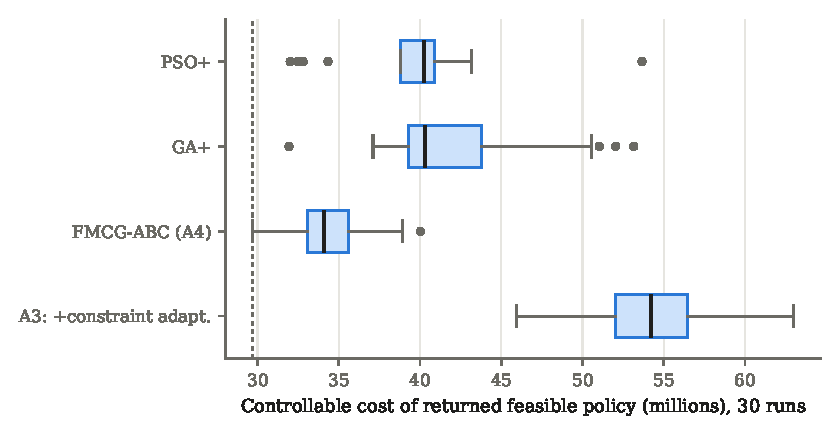
\includegraphics[width=0.78\linewidth]{generated/fig_cost_box.pdf}
\caption{Distribution over 30 runs of the controllable cost of the returned feasible policy, main instance. Dashed line: best known feasible solution.}\label{fig:box}
\end{figure}

Table~\ref{tab:stats} reports the statistical comparison. Across the four methods that were feasible in all runs, the Kruskal--Wallis test rejects equal distributions ($H=83.9$, $p<10^{-4}$). The medians of FMCG-ABC were lower than those of A3, GA+ and PSO+ by 20.11, 6.20 and 6.12 million, with bootstrap confidence intervals that exclude zero; all three Mann--Whitney tests remain significant after Holm correction ($p<10^{-4}$). A randomly chosen FMCG-ABC run was cheaper than a randomly chosen run of A3, GA+ and PSO+ with probability $A_{12}=1.00$, 0.95 and 0.81: the advantage over PSO+ is clear but not uniform. Methods that were infeasible in some runs were not tested on cost.

\begin{table}[!htbp]
\centering
\footnotesize
\caption{Comparison of FMCG-ABC with each method feasible in all runs on the main instance (two-sided Mann--Whitney U test on controllable cost, Holm correction; runs of different methods are independent).}\label{tab:stats}
\resizebox{\linewidth}{!}{%
\begin{tabular}{lrrrrrr}
\toprule
Comparison & $n$ & $U$ & $p$ & $p_{\mathrm{Holm}}$ & Diff.\ of medians [95\% CI] & $A_{12}$ \\
\midrule
FMCG-ABC vs A3 & 30/30 & 0 & $<10^{-4}$ & $<10^{-4}$ & -20.11 [-21.57, -18.79] & 1.00 \\
FMCG-ABC vs GA+ & 30/30 & 43 & $<10^{-4}$ & $<10^{-4}$ & -6.20 [-7.80, -5.28] & 0.95 \\
FMCG-ABC vs PSO+ & 30/30 & 172 & $<10^{-4}$ & $<10^{-4}$ & -6.12 [-6.93, -4.84] & 0.81 \\
\bottomrule
\end{tabular}}
\par\smallskip\parbox{0.95\linewidth}{\scriptsize Difference of medians: FMCG-ABC minus comparator, millions; negative favours FMCG-ABC; CI: percentile bootstrap of both groups independently (5000 resamples). $A_{12}$: probability that a randomly chosen FMCG-ABC run is cheaper than a randomly chosen comparator run (Vargha--Delaney). Kruskal--Wallis test across the four methods: $H=83.9$, $p<10^{-4}$.}
\end{table}


\subsection{How far from optimal? (E1--E3)}\label{sec:res-gap}
The Lagrangian lower bound for the main instance is 25.02 million; the BKS is 18.7\% above it and the FMCG-ABC median 36.3\% above it. Because the instance has quantity discounts, the bound is not tight, and these percentages are upper bounds on the true gaps rather than estimates. E2 and E3 measure the gaps exactly (Table~\ref{tab:exact}).

\begin{table}[!htbp]
\centering
\footnotesize
\caption{Gaps to a certified optimum: (a) main instance without quantity discounts (convex; optimum certified by the Lagrangian dual, duality gap 0.0000\%); (b) five 6-SKU instances with discounts (optimum by enumerating all $2^6$ price regimes).}\label{tab:exact}
\resizebox{\linewidth}{!}{%
\begin{tabular}{lrrrrrr}
\toprule
Method & \multicolumn{3}{c}{(a) $N=50$, convex} & \multicolumn{3}{c}{(b) $N=6$, discounts} \\ \cmidrule(lr){2-4}\cmidrule(lr){5-7} & Feas. (\%) & Median gap & Max gap & Feas. (\%) & Median gap & Max gap \\
\midrule
GA & 10 & 49.96 & 49.96 & 100 & 11.58 & 48.12 \\
PSO & 0 & -- & -- & 100 & 47.29 & 131.26 \\
ABC (A1) & 0 & -- & -- & 100 & 17.50 & 63.85 \\
FMCG-ABC (A4) & 100 & 0.10 & 0.11 & 100 & 7.85 & 47.30 \\
GA+ & 100 & 0.10 & 0.15 & 100 & 7.66 & 47.39 \\
PSO+ & 100 & 0.17 & 0.22 & 100 & 7.61 & 47.29 \\
\bottomrule
\end{tabular}}
\par\smallskip\parbox{0.95\linewidth}{\scriptsize Gap $=(TC-TC^{*})/(TC^{*}-C_0)\times100$ on feasible runs, $C_0=\sum_i D_i\min(p^{reg}_i,p^{disc}_i)$. (a) 10 runs per method, $E_{\max}$ as in Table~\ref{tab:e1}; (b) 10 runs per instance, $E_{\max}=10{,}000$.}
\end{table}


Without discounts (E2) the bound and the best dual-recovered primal policy coincide (duality gap $10^{-6}$\%), so the optimum is certified. The three adapted methods then came within 0.10\% (FMCG-ABC, GA+) and 0.17\% (PSO+) of the optimum in median, while penalty-based PSO and ABC returned no feasible policy and GA one policy 50\% above the optimum. On the five small discounted instances (E3) all methods were feasible, and the three adapted methods had almost identical median gaps (PSO+ 7.6\%, GA+ 7.7\%, FMCG-ABC 7.9\%); FMCG-ABC had the lowest per-instance median on three of the five instances. Their worst runs were 47\% above the optimum, and the generic methods were further away. To find the cause, we solved each instance separately for every price-regime combination and re-ran the adapted methods (10 seeds each): 135 of 150 runs ended in a suboptimal combination of regimes, 104 of the 106 runs with a gap above 5\% did so, and within the regime they selected, the runs were a median 0.15\% from that regime's optimum. Together with E2, this locates the hardness of the model in the discrete choice of price regimes rather than in the continuous part, which the adapted methods solve almost exactly.\footnote{The exact references of E3 were first computed with an unscaled sequential quadratic programming solver; because some heuristic runs then beat the reported ``optimum'', which is impossible, the references were recomputed with a scaled formulation from six starting points. After the correction no run beats the reference (smallest gap 0.04\%), and the per-regime Lagrangian bounds of S1 certify every corrected reference to within $2\times10^{-6}$\% of controllable cost, so they are optimal to numerical precision. The heuristic runs did not depend on the reference and were not repeated.}

\subsection{Which adaptation matters? (ablation)}\label{sec:res-ablation}
Table~\ref{tab:ablation} adds the adaptations one at a time. EOQ-informed initialisation (A2) raised the number of feasible runs from 1 to 21 of 30 and lowered the median feasible cost from 80.5 to 60.9 million, but still left infeasible runs, because a penalised search can drift away from a feasible start. The inventory-specific constraint handling (A3: service-as-bound, repair and feasibility-first ranking) made every run feasible and lowered the median to 54.2 million. The log-scale multi-dimensional move (A4) produced the largest single improvement, to 34.1 million. The same constraint handling also made GA and PSO competitive (GA+, PSO+), so the constraint adaptations are not specific to ABC; what distinguished FMCG-ABC from the adapted GA and PSO in E1 is the combination with the perturbation scheme.

\begin{table}[!htbp]
\centering
\footnotesize
\caption{Ablation of the FMCG-specific adaptations (main instance).}\label{tab:ablation}
\resizebox{\linewidth}{!}{%
\begin{tabular}{lrrrrrr}
\toprule
Configuration & Feasible & Median & $\Delta_{\mathrm{BKS}}$ (\%) & Med. viol. (\%) & Realised CSL (\%) & Fill (\%) \\
\midrule
ABC (A1) & 1/30 & 80.51 & 171.0 & 0.74 & 97.8 & 99.59 \\
A2: +EOQ init. & 21/30 & 60.93 & 105.1 & 0.00 & 96.3 & 99.61 \\
A3: +constraint adapt. & 30/30 & 54.21 & 82.5 & 0.00 & 94.7 & 99.68 \\
FMCG-ABC (A4) & 30/30 & 34.10 & 14.8 & 0.00 & 92.9 & 99.34 \\
\bottomrule
\end{tabular}}
\par\smallskip\parbox{0.95\linewidth}{\scriptsize Median cost over feasible runs (millions; -- if none). Median violation: normalised aggregate violation of the returned solution. Realised CSL and fill rate: holdout replay of the median run (Table~\ref{tab:replay}); for A1 the median run is infeasible, so its replay describes an inadmissible policy.}
\end{table}


\subsection{Convergence}
Figure~\ref{fig:conv} shows the best feasible cost against the number of evaluations (median and interquartile band over 30 runs). PSO+ improved fastest initially and led until about 10{,}000 evaluations, after which it stagnated near 40 million; FMCG-ABC kept improving until the end of the budget. The curves are still decreasing at 50{,}000 evaluations, so all methods would benefit from a larger budget, and the ranking at a much smaller budget would differ.

\begin{figure}[!htbp]
\centering
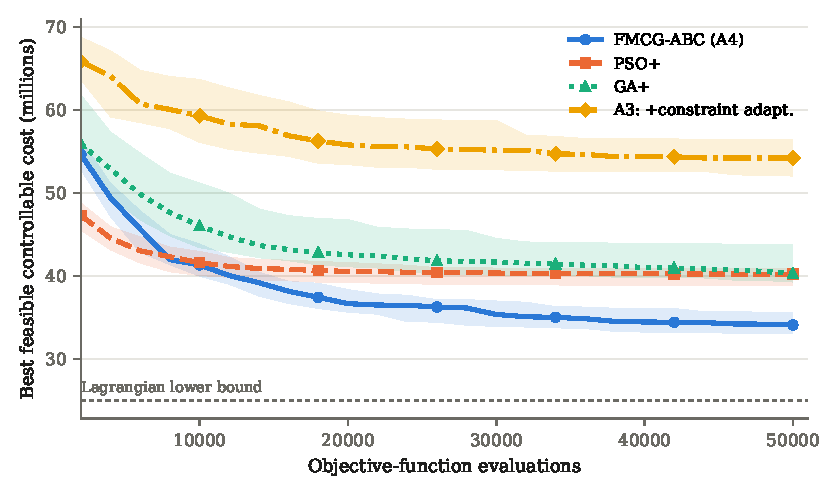
\includegraphics[width=0.85\linewidth]{generated/fig_convergence.pdf}
\caption{Best feasible controllable cost versus objective evaluations on the main instance (line: median of 30 runs; band: interquartile range). Dashed: Lagrangian lower bound.}\label{fig:conv}
\end{figure}

\subsection{Equal wall-clock time (X1)}\label{sec:res-time}
Because our ABC implementation evaluates and repairs one candidate at a time, whereas GA and PSO evaluate whole populations in vectorised form, FMCG-ABC needed about 32 seconds per run on the main instance against 2 seconds for PSO+ and 3 seconds for GA+. To check whether the ranking depends on the equal-evaluation criterion, we gave PSO+ and GA+ the number of evaluations they can perform in the time FMCG-ABC needs for 50{,}000 (952{,}752 and 478{,}667 evaluations; Table~\ref{tab:x1}). With 10 to 19 times more evaluations, and in practice slightly more time than FMCG-ABC, both remained more expensive: median controllable cost 40.24 (PSO+) and 38.35 million (GA+) against 34.00 million, The difference to GA+ is significant (Mann--Whitney, Holm-adjusted $p<0.001$, $A_{12}=1.00$); the difference to PSO+ is not ($p=0.064$, $A_{12}=0.75$, and the confidence interval of the difference of medians, $[-7.59,+1.65]$ million, includes zero). With ten independent runs per method, we therefore conclude that FMCG-ABC was not worse than PSO+ at equal time and better than GA+, not that its advantage over PSO+ survives equal time; the additional evaluations did not move PSO+ and GA+ in median away from the region where they stagnate (Figure~\ref{fig:conv}).

\begin{table}[!htbp]
\centering
\footnotesize
\caption{Equal wall-clock time (X1): adapted GA and PSO receive the number of evaluations they can perform in the mean time FMCG-ABC needs for 50{,}000 evaluations; seeds 1--10, main instance.}\label{tab:x1}
\resizebox{\linewidth}{!}{%
\begin{tabular}{lrrrrrrrr}
\toprule
Comparator & Evaluations & Feasible & FMCG-ABC & Comparator & Time (s) & Diff.\ of medians, 95\% CI & $p_{\mathrm{Holm}}$ & $A_{12}$ \\
\midrule
PSO+ & 952,752 & 10/10 & 34.00 & 40.24 & 32 / 46 & [-7.59, +1.65] & 0.0640 & 0.75 \\
GA+ & 478,667 & 10/10 & 34.00 & 38.35 & 32 / 44 & [-6.62, -3.50] & 0.0004 & 1.00 \\
\bottomrule
\end{tabular}}
\par\smallskip\parbox{0.95\linewidth}{\scriptsize Median controllable cost (millions); FMCG-ABC values are its E1 runs with the same seeds. Time: mean seconds per run, FMCG-ABC / comparator. Runs are independent samples (10 per method): two-sided Mann--Whitney U test with Holm correction, Vargha--Delaney $A_{12}$, bootstrap 95\% CI of the difference of medians.}
\end{table}


\subsection{Robustness and scalability (E4, E5, X2, X3)}\label{sec:res-robust}
Across five further 50-SKU instances with five runs each (Table~\ref{tab:robust}), FMCG-ABC had the lowest median gap to the best solution found for each instance at tight resources (4.7\% vs.\ 10.3\% for PSO+ and 13.4\% for GA+) and at loose resources (5.5\% vs.\ 14.1\% and 19.1\%). It attained the best solution in 4 of 25 runs at tight resources, but at loose resources PSO+ did so more often (3 vs.\ 1 of 25 runs), so the median advantage does not mean that FMCG-ABC finds the best policy most often. Standard ABC was never feasible at tight resources and feasible in 5 of 25 runs at loose resources.

\begin{table}[!htbp]
\centering
\footnotesize
\caption{Robustness across five independently generated 50-SKU instances at tight ($\tau=0.60$) and loose ($\tau=0.90$) coupling constraints (5 runs per instance and method; E4 extended by X3).}\label{tab:robust}
\resizebox{\linewidth}{!}{%
\begin{tabular}{lrrrrrr}
\toprule
Method & \multicolumn{3}{c}{$\tau=0.60$} & \multicolumn{3}{c}{$\tau=0.90$} \\ \cmidrule(lr){2-4}\cmidrule(lr){5-7} & Feas. (\%) & Med. $\Delta_{\mathrm{best}}$ (\%) & Wins & Feas. (\%) & Med. $\Delta_{\mathrm{best}}$ (\%) & Wins \\
\midrule
ABC (A1) & 0 & -- & 0 & 20 & 124.8 & 0 \\
FMCG-ABC (A4) & 100 & 4.7 & 4 & 100 & 5.5 & 1 \\
GA+ & 100 & 13.4 & 0 & 100 & 19.1 & 1 \\
PSO+ & 100 & 10.3 & 1 & 100 & 14.1 & 3 \\
\bottomrule
\end{tabular}}
\par\smallskip\parbox{0.95\linewidth}{\scriptsize $\Delta_{\mathrm{best}}$: gap to the best feasible cost found for that instance by any method; Wins: runs attaining it (out of 25).}
\end{table}


For scalability we used three generated instances per size and five runs per instance (Table~\ref{tab:scal}, Figure~\ref{fig:scal}). FMCG-ABC had the lowest median gap for $N=50$, 75 and 100 (4.2\%, 5.3\% and 4.9\%), but not for $N=25$, where PSO+ was ahead (8.3\% vs.\ 10.9\%). Standard ABC was feasible only for $N=25$. An earlier single-instance version of this experiment (E5, 10 runs) had ranked GA+ first for $N=100$; the three-instance results show that this ranking was specific to that instance, which is why we report the extended design. Runtime grows with $N$ for all methods, and FMCG-ABC remained the slowest per evaluation.

\begin{table}[!htbp]
\centering
\footnotesize
\caption{Scalability: median gap to the best feasible solution of each instance, over three generated instances per size and 5 runs each (E5 extended by X2), and mean runtime per run.}\label{tab:scal}
\resizebox{\linewidth}{!}{%
\begin{tabular}{lrrrrrrrr}
\toprule
Method & \multicolumn{2}{c}{$N=25$} & \multicolumn{2}{c}{$N=50$} & \multicolumn{2}{c}{$N=75$} & \multicolumn{2}{c}{$N=100$} \\ \cmidrule(lr){2-3}\cmidrule(lr){4-5}\cmidrule(lr){6-7}\cmidrule(lr){8-9} & $\Delta_{\mathrm{best}}$ (\%) & s & $\Delta_{\mathrm{best}}$ (\%) & s & $\Delta_{\mathrm{best}}$ (\%) & s & $\Delta_{\mathrm{best}}$ (\%) & s \\
\midrule
ABC (A1) & 60.9 & 13 & infeas. & 14 & infeas. & 14 & infeas. & 14 \\
FMCG-ABC (A4) & 10.9 & 39 & 4.2 & 48 & 5.3 & 51 & 4.9 & 53 \\
GA+ & 12.7 & 4 & 13.0 & 4 & 14.2 & 5 & 11.6 & 6 \\
PSO+ & 8.3 & 2 & 9.1 & 2 & 7.0 & 3 & 7.8 & 3 \\
\bottomrule
\end{tabular}}
\par\smallskip\parbox{0.95\linewidth}{\scriptsize Runtimes were measured with two runs in parallel on two cores and include repair; they are comparable within a column only.}
\end{table}


\begin{figure}[!htbp]
\centering
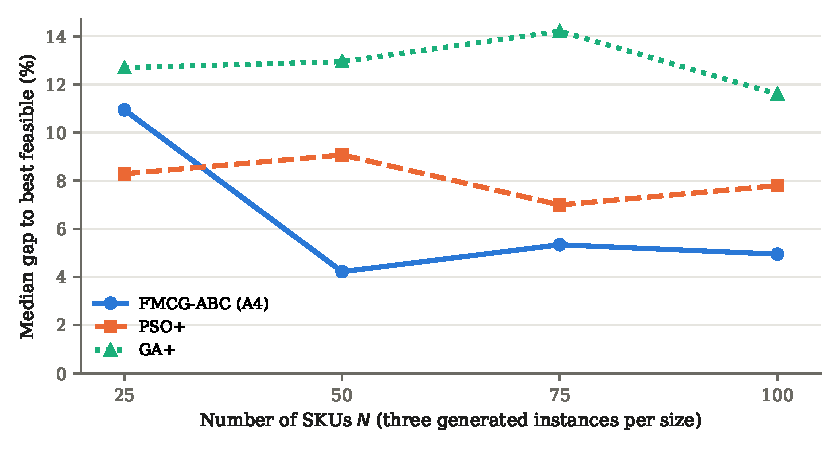
\includegraphics[width=0.78\linewidth]{generated/fig_scalability.pdf}
\caption{Median gap to the best feasible solution per instance size (three instances per size, five runs each).}\label{fig:scal}
\end{figure}

\subsection{Sensitivity (E6, X4)}\label{sec:res-sens}
Table~\ref{tab:sens} reports the re-optimised FMCG-ABC policy cost for one-at-a-time parameter changes, with ten runs per scenario and the sensitivity index of equation~(\ref{eq:si}) on controllable cost. On total cost every change is below 0.5\%, because purchasing dominates $TC$. On controllable cost, a 10\% tighter warehouse capacity raised the cost by 18.5\%, a 10\% tighter budget by 14.4\% and a one-point higher service target by 11.4\%, while a 10\% larger budget lowered it by 16.8\%; a 10\% larger capacity and a three-point lower service target lowered it by about 5\%. Demand variability moved it by $-3.2\%$ ($\sigma_d\times0.8$) and $+7.0\%$ ($\sigma_d\times1.2$). The resource effects exceed the run-to-run variability of FMCG-ABC (interquartile range 7\% of the median) and agree in sign with the change of the lower bound (Section~\ref{sec:artifact}); the demand-variability effects are of the order of that variability. On this portfolio, the binding resources and the service targets drive the cost of the policy more than demand variability does.

\begin{table}[!htbp]
\centering
\footnotesize
\caption{Sensitivity of the re-optimised FMCG-ABC policy cost to model parameters (10 runs per scenario; E6 extended by X4).}\label{tab:sens}
\begin{tabular}{lrrrr}
\toprule
Scenario & Feas. (\%) & Median ctrl. cost & IQR & $SI^{ctrl}$ (\%) \\
\midrule
$\sigma_d\times0.8$ & 100 & 33.01 & [31.73, 34.63] & -3.2 \\
$\sigma_d\times1.2$ & 100 & 36.48 & [34.93, 37.91] & +7.0 \\
$\alpha_i-0.03$ & 100 & 32.52 & [32.04, 33.17] & -4.6 \\
$\alpha_i+0.01$ & 100 & 37.99 & [35.70, 38.92] & +11.4 \\
$B\times0.9$ & 100 & 39.00 & [37.65, 40.33] & +14.4 \\
$B\times1.1$ & 100 & 28.39 & [28.14, 29.67] & -16.8 \\
$Cap_w\times0.9$ & 100 & 40.41 & [39.50, 41.17] & +18.5 \\
$Cap_w\times1.1$ & 100 & 32.44 & [32.11, 32.94] & -4.9 \\
\bottomrule
\end{tabular}
\par\smallskip\parbox{0.95\linewidth}{\scriptsize $SI^{ctrl}$: change of the median controllable cost relative to the median of the 30 E1 runs (34.10 million), eq.~(\ref{eq:si}). Base run-to-run IQR: 2.52 million (7.4\%).}
\end{table}


\subsection{Out-of-sample service (E7)}\label{sec:replay}
Table~\ref{tab:replay} reports the replay of each method's median policy on the 270-day holdout. All feasible policies met their targets on average in the model (mean model-implied CSL 95.0--96.4\% against a mean target of 93.1\%), but realised CSL was lower: 92.9\% for FMCG-ABC, 92.3\% for PSO+, 94.8\% for GA+ and 94.7\% for A3, with 25 to 28 of the 50 SKUs below their individual targets. Fill rates remained above 99.3\%. The EOQ policy realised 90.5\% with 38 SKUs below target. Cycle service level and fill rate measure different things: a stockout that is cleared within a day hardly affects the fill rate but makes the whole cycle a failure, so a high portfolio fill rate does not imply that every SKU meets its cycle-service target.

To explain the shortfall we replayed the median FMCG-ABC policy under variants (S3, Table~\ref{tab:s3}). Replacing the Gamma holdout by normal demand with the calibrated mean and standard deviation did not remove the shortfall (realised CSL 91.7\%, 28 SKUs below target), so the non-normality of demand is not its main cause. Adding to each reorder point the expected undershoot of daily review, $(\sigma_{d,i}^2+d_i^2)/(2d_i)$, which the continuous-review model ignores, raised the realised CSL to 95.3\% and reduced the SKUs below target from 27 to 17, at 2{,}562 additional units of safety stock and 0.54 million of additional holding cost. The corrected policy, however, needs 105.4\% of the capacity of the second warehouse and is therefore infeasible: the allowance must be built into the model and re-optimised, not added afterwards (Section~\ref{sec:res-variants}). The 17 remaining shortfalls indicate further sources that we did not isolate, such as integer lead times and the short holdout. Policies with less safety stock above the service requirement are the most exposed: FMCG-ABC and PSO+, whose mean model-implied CSL (95.0\% and 95.5\%) is closer to the targets than that of GA+ and A3 (96.3\% and 96.4\%), show the larger shortfall. Model feasibility is therefore necessary but not sufficient for service, which is why the artifact reports realised service next to the model-implied value and rule R1 fires when they diverge.

\begin{table}[!htbp]
\centering\footnotesize
\caption{Replay diagnostic for the median FMCG-ABC policy (S3; 30 lead-time replications each).}\label{tab:s3}
\resizebox{\linewidth}{!}{%
\begin{tabular}{lrrr}
\toprule
Variant & Realised CSL (\%) & Fill rate (\%) & SKUs $<\alpha_i$ \\
\midrule
(a) Gamma holdout (as in Table~\ref{tab:replay}) & 92.9 & 99.34 & 27 \\
(b) Normal demand, calibrated mean and s.d. & 91.7 & 99.45 & 28 \\
(c) Gamma holdout + undershoot allowance & 95.3 & 99.61 & 17 \\
(d) Normal demand + undershoot allowance & 95.1 & 99.71 & 14 \\
\bottomrule
\end{tabular}}
\par\smallskip\parbox{0.95\linewidth}{\scriptsize Allowance $(\sigma_{d,i}^2+d_i^2)/(2d_i)$ added to $SS_i$; variants (c) and (d) exceed the capacity of warehouse 2 (105.4\%) and are diagnostics, not admissible policies.}
\end{table}

\begin{table}[!htbp]
\centering
\footnotesize
\caption{Out-of-sample replay of the median run of each method on the 270-day holdout demand (30 lead-time replications; daily review; backorders).}\label{tab:replay}
\resizebox{\linewidth}{!}{%
\begin{tabular}{lrrrrrrr}
\toprule
Method & Feasible & Model CSL & Realised CSL [95\% CI] & Fill rate & Short. units/yr & SKUs $<\alpha_i$ & Ctrl. cost \\
\midrule
EOQ + static SS & no & 93.1 & 90.5 [90.2, 90.9] & 99.48 & 7,996 & 38 & 17.47 \\
GA & no & 97.6 & 97.3 [97.2, 97.4] & 99.31 & 10,572 & 11 & 28.31 \\
PSO & no & 87.0 & 79.4 [79.2, 79.6] & 83.05 & 259,384 & 15 & 162.42 \\
ABC (A1) & no & 96.7 & 97.8 [97.7, 97.9] & 99.59 & 6,264 & 17 & 25.99 \\
FMCG-ABC (A4) & yes & 95.0 & 92.9 [92.6, 93.1] & 99.34 & 10,052 & 27 & 19.09 \\
GA+ & yes & 96.3 & 94.8 [94.6, 95.0] & 99.62 & 5,782 & 25 & 17.04 \\
PSO+ & yes & 95.5 & 92.3 [92.0, 92.6] & 99.48 & 7,943 & 28 & 17.21 \\
\bottomrule
\end{tabular}}
\par\smallskip\parbox{0.95\linewidth}{\scriptsize Model CSL: mean of $\Phi(z_i)$ (eq.~\ref{eq:cslmodel}); mean target $\bar\alpha=93.1\%$. Realised controllable cost excludes purchasing (millions). Demand in the holdout is Gamma-distributed, not normal.}
\end{table}


\subsection{Model variants (X5, X6)}\label{sec:res-variants}
Table~\ref{tab:variants} repeats the main comparison under two variants of the model. With the budget defined as the average capital tied up in stock (X5), the budget is the only binding resource at the dual solution (warehouse multipliers zero); all three adapted methods remained feasible in every run and standard ABC in none, and FMCG-ABC again had the lowest median controllable cost (53.64 million, against 56.56 for GA+ and 63.22 for PSO+) and the smallest dispersion. The conclusions of the comparison therefore do not depend on which budget definition is adopted, although the cost levels do.

With the daily-review undershoot built into the service constraint and the shortage cost (X6), the re-optimised FMCG-ABC policy cost 35.42 million, 3.9\% more than under the continuous-review model, and raised the realised cycle service level on the holdout from 92.9\% to 96.8\%, with 9 instead of 27 SKUs below their targets; GA+ and PSO+ reached 96.5\% and 95.9\%. Unlike the post-hoc allowance of S3, these policies respect the warehouse capacities. Most of the out-of-sample service shortfall reported above is thus removed by modelling the review period, at a modest increase of controllable cost. The variant is not uniformly better: it assumes that the review period stays daily, uses an approximation of the expected undershoot, still leaves 9 SKUs below target, and costs 1.3 million more per year; whether that is worthwhile depends on how the firm values the avoided stockouts beyond the shortage cost already in the model. It is therefore offered to planners as an alternative policy with its cost and service consequences, not as a replacement.

\begin{table}[!htbp]
\centering
\footnotesize
\caption{Model variants on the main instance (10 runs per method): budget as average capital tied up in stock (X5) and daily-review undershoot inside the model (X6).}\label{tab:variants}
\resizebox{\linewidth}{!}{%
\begin{tabular}{llrrrrrr}
\toprule
Variant & Method & Feasible & Median ctrl. & IQR & Lower bound & Realised CSL (\%) & SKUs $<\alpha_i$ \\
\midrule
Average-investment budget & ABC (A1) & 0/10 & -- & -- & 37.10 & -- & -- \\
 & FMCG-ABC (A4) & 10/10 & 53.64 & 1.29 &  & -- & -- \\
 & GA+ & 10/10 & 56.56 & 8.62 &  & -- & -- \\
 & PSO+ & 10/10 & 63.22 & 8.94 &  & -- & -- \\
Daily-review model & FMCG-ABC (A4) & 10/10 & 35.42 & 3.73 & 25.63 & 96.8 & 9 \\
 & GA+ & 10/10 & 42.99 & 2.44 &  & 96.5 & 9 \\
 & PSO+ & 10/10 & 41.26 & 0.88 &  & 95.9 & 16 \\
\bottomrule
\end{tabular}}
\par\smallskip\parbox{0.95\linewidth}{\scriptsize Millions of currency units. X5: $B=0.75\sum_ip_i(Q^{EOQ}_i)(Q^{EOQ}_i/2+SS_i)$. X6: offset $u_i=(\sigma_{d,i}^2+d_i^2)/(2d_i)$ in the service constraint and the shortage cost; realised service from the replay of the median run (main model, E1: FMCG-ABC 92.9\%, 27 SKUs below target).}
\end{table}


